\begin{center}
    \captionof{figure}{Within- and Between-Person Effects of Binary Predictor and Outcome}

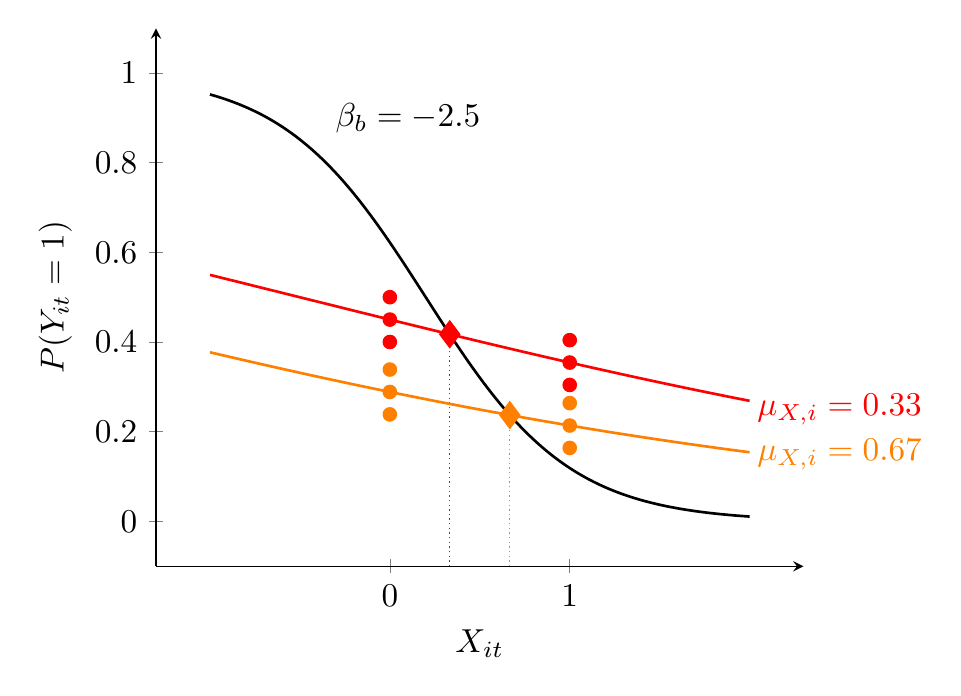
\begin{tikzpicture}[scale=1.2]
    \begin{axis}[
        axis x line=left, axis y line=left,
        xlabel={$X_{it}$}, ylabel={$P(Y_{it} = 1)$},
        xmin=-1, xmax=2, ymin=0, ymax=1,
        % legend pos=south west,
        samples=200,
        domain=-1:2,
        ytick={0,0.2,0.4,0.6,0.8,1},
        xtick={0,1},
        clip=false,
        enlargelimits=true
    ]
    
    % Parameters
    \pgfmathsetmacro{\gammaZero}{0.5}
    \pgfmathsetmacro{\gammaOne}{-2.1}
    \pgfmathsetmacro{\betaOne}{-0.4}
    \pgfmathsetmacro{\betaB}{-2.5}
    
    % Person 1: mu_X = 0.333
    \pgfmathsetmacro{\muXone}{0.333}
    \pgfmathsetmacro{\intOne}{\gammaZero + \gammaOne*\muXone}
    \addplot[red, thick] {1 / (1 + exp(-(\intOne + \betaOne*x)))};
    \addplot[only marks, mark=diamond*, mark size=4pt, red] coordinates {
        (0.333, {1 / (1 + exp(-(\intOne + \betaOne*0.333)))})
    };
    \addplot[only marks, mark=*, red] coordinates {
        (0, {1 / (1 + exp(-(\intOne + \betaOne*0)))})
        (0, {1 / (1 + exp(-(\intOne + \betaOne*0))) + 0.05})
        (0, {1 / (1 + exp(-(\intOne + \betaOne*0))) - 0.05})
        (1, {1 / (1 + exp(-(\intOne + \betaOne*1)))})
        (1, {1 / (1 + exp(-(\intOne + \betaOne*1))) + 0.05})
        (1, {1 / (1 + exp(-(\intOne + \betaOne*1))) - 0.05})
    };
    \addplot[densely dotted, thin, red] coordinates {
        (\muXone, -0.1)
        (\muXone, {1 / (1 + exp(-(\intOne + \betaOne*\muXone)))})
    };
    
    % Person 2: mu_X = 0.667
    \pgfmathsetmacro{\muXtwo}{0.667}
    \pgfmathsetmacro{\intTwo}{\gammaZero + \gammaOne*\muXtwo}
    \addplot[orange, thick] {1 / (1 + exp(-(\intTwo + \betaOne*x)))};
    \addplot[only marks, mark=diamond*, mark size=4pt, orange] coordinates {
        (0.667, {1 / (1 + exp(-(\intTwo + \betaOne*0.667)))})
    };
    \addplot[only marks, mark=*, orange] coordinates {
        (0, {1 / (1 + exp(-(\intTwo + \betaOne*0)))})
        (0, {1 / (1 + exp(-(\intTwo + \betaOne*0))) + 0.05})
        (0, {1 / (1 + exp(-(\intTwo + \betaOne*0))) - 0.05})
        (1, {1 / (1 + exp(-(\intTwo + \betaOne*1)))})
        (1, {1 / (1 + exp(-(\intTwo + \betaOne*1))) + 0.05})
        (1, {1 / (1 + exp(-(\intTwo + \betaOne*1))) - 0.05})
    };
    
    \addplot[densely dotted, thin, orange] coordinates {
    (\muXtwo, -0.1)
    (\muXtwo, {1 / (1 + exp(-(\intTwo + \betaOne*\muXtwo)))})
    };
    
    % Between-person curve
    \addplot[black, thick] {1 / (1 + exp(-(\gammaZero + \betaB*x)))};

    % === Labels ===
    \node[red] at (axis cs:2.5,0.25){$\mu_{X,i}=0.33$};
    \node[orange] at (axis cs:2.5,0.15) {$\mu_{X,i}=0.67$};
    \node[black] at (axis cs:0.1,0.9) {$\beta_\text{b} = -2.5$};
    
    \end{axis}
\end{tikzpicture}

    \label{fig:withinbetween-binxy}
    \begin{figurenote}
        The solid black slope represents the between-person effect and the colored slopes the within-cluster effects. The X-axis simultaneously represents $X_{it}$ for the within-slope and $\mu_{X,i}$ for the between-slope; and the Y-axis represents $Y_{it}$ for the within slope and $Y_i$ for the between-slope. Dots reflect possible datapoints and diamonds reflect the position of $\mu_{X,i}$ on the within-person slope.
    \end{figurenote}
\end{center}